\documentclass[12pt]{article}
\usepackage[top=1in, bottom=1in, left=1in, right=1in]{geometry}
%\usepackage[margin=1in]{geometry}
\usepackage[onehalfspacing]{setspace}
%\usepackage[doublespacing]{setspace}
\usepackage{amsmath, amssymb, amsthm}
\usepackage{enumerate, enumitem}
\usepackage{fancyhdr, graphicx, proof, comment, multicol}
\usepackage[none]{hyphenat} % This command prevents hyphenation of words
\binoppenalty=\maxdimen % This command and the next prevent in-line equation breaks
\relpenalty=\maxdimen
%    Good website with common symbols
% http://www.artofproblemsolving.com/wiki/index.php/LaTeX%3ASymbols
%    How to change enumeration using enumitem package
% http://tex.stackexchange.com/questions/129951/enumerate-tag-using-the-alphabet-instead-of-numbers
%    Quick post on headers
% http://timmurphy.org/2010/08/07/headers-and-footers-in-latex-using-fancyhdr/
%    Info on alignat
% http://tex.stackexchange.com/questions/229799/align-words-next-to-the-numbering
% http://tex.stackexchange.com/questions/43102/how-to-subtract-two-equations
%    Text align left-center-right
% http://tex.stackexchange.com/questions/55472/how-to-make-text-aligned-left-center-right-in-the-same-line
\usepackage{microtype} % Modifies spacing between letters and words
\usepackage{mathpazo} % Modifies font. Optional package.
\usepackage{mdframed} % Required for boxed problems.
\usepackage{parskip} % Left justifies new paragraphs.
\linespread{1.1} 


%figure support
\usepackage{import}
\usepackage{xifthen}
\pdfminorversion=7
\usepackage{pdfpages}
\usepackage{transparent}
\newcommand{\incfig}[1]{%
	\def\svgwidth{\columnwidth}
	\import{./figures/}{#1.pdf_tex}
}
\graphicspath{ {./figures/} }
\pdfsuppresswarningpagegroup=1

\newenvironment{problem}[1]
{\begin{mdframed}[linewidth=0.8pt]
        \textsc{Problem #1:}

}
    {\end{mdframed}}

\newenvironment{solution}
    {\textsc{Solution:}\\}
    {\newpage}% puts a new page after the solution
    
\newenvironment{statement}[1]
{\begin{mdframed}[linewidth=0.6pt]
        \textsc{Statement #1:}

}
    {\end{mdframed}}

%\newenvironment{prf}
 %   {\textsc{Proof:}\\}
 %   {\newpage}% puts a new page after the solution

\begin{document}
% This is the Header
% Make sure you update this information!!!!
\noindent
\textbf{CIS4367.01} \hfill \textbf{Brandon Thompson} \\
\normalsize Prof. Elibol \hfill Due Date: 2/28/2020 \\

% This is where you name your homework
\begin{center}
\textbf{Homework 7}
\end{center}
	\begin{problem}{}
		Research the 2013 Target data breach and prepare a report about the attack.
		Provide the following:
		\begin{itemize}
			\item Brief description of the attack.
			\item Timeline of the attack.
			\item Root cause analysis. What happened? How it happened? (Technical analysis).
			\item Discussion of how the company became aware of the breach.
			\item What were the consequences of the breach? Effects of the breach (Reputational? Financial? Operational?)
			\item Are there any lessons learned?
			\item Discuss breach in terms of confidentiality, integrity, and availability in general.
		\end{itemize}
	\end{problem}
	\begin{solution}
		In 2013 Target notified 110 million shoppers that their personal and financial information
		had been compromised. The attack started on November 27, 2013 (Black Friday) and Target
		notified the US	Justice Department by December 13. By December 15th, Target had a third party
		forensic team in place and the attack mitigated.
		\begin{figure}[ht!]
			\centering
			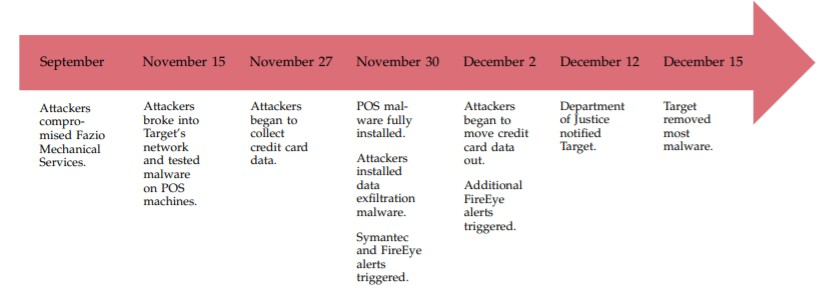
\includegraphics[width=0.8\textwidth]{target_attack_timeline}
			\caption{Timeline of the Target data breach (Shu et al.)}
			\label{fig:timeline}
		\end{figure}
		\textbf{Gathering information:} We do not know how attackers were able to gather information
		about Target's network before the attack, however there is a plethora of information about
		supplier interaction and Microsoft management systems for security patches.

		\textbf{Compromise system:} Target's network was to well protected, being the large
		corporation that they are. Third party vendors, however, do not have as many resources.
		An employee at Fazio Mechanical was duped in a phishing email that installed \texttt{Citadel},
		a banking trojan on Fazio computers. Attackers then had to wait for the vendors Target
		portal login.

		\textbf{After vendor access:} Target has not released this information but it is possible that
		attackers used SQL injection, XSS or a 0-day attack on the web application to elevate
		privileges and then access internal systems.

		\textbf{Internal Servers:} Speculated that attackers used an attack cycle
		in \texttt{Mandiant's APT1 report} defined by Figure ~\ref{fig:attack_lifecycle_model} to move laterally through the network.
		\begin{figure}[ht!]
			\centering
			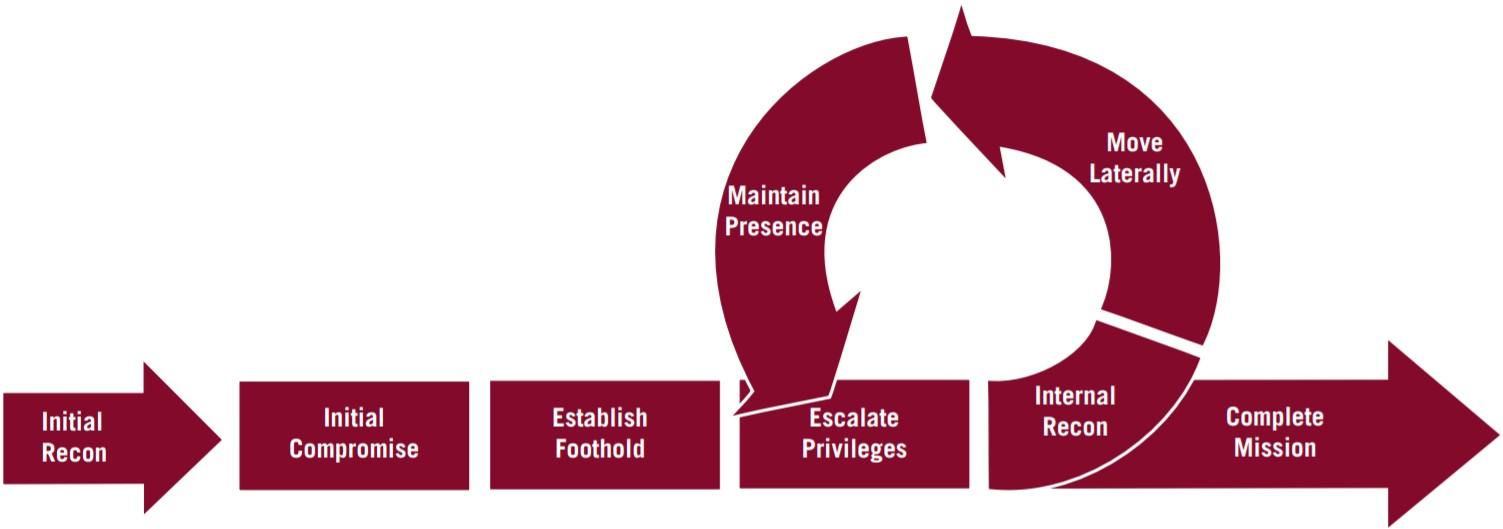
\includegraphics[width=0.8\textwidth]{attack_lifecycle_model}
			\caption{Mandiant's Attack Lifecycle Model (Page 27 of Mandiant APT1 report).}
			\label{fig:attack_lifecycle_model}
		\end{figure}
		
		\textbf{Point of Sale Systems:} Malware code utilized RAM-scraping to grab card information
		from memory of POS-devices. Malware checks if time is between 10AM and 5PM to send
		a \texttt{winxml.dll} file over a temporary NetBIOS share to an internal dump server
		within the network. Meaning POS systems that were not able to access the internet
		were still vulnerable. Attackers the moved stolen data off-site.

		Target was made aware of errors in their system by their FireEye security system but chose
		to ignore the initial warning. Later flags revealed a much larger problem than was
		originally thought.

		\textbf{Lessons Learned:}
		\begin{itemize}
			\item Monitor system activity more closely.
			\item Implement POS management tools.
			\item Least privilege on vendor accounts.
			\item Two-factor authentication.
		\end{itemize}
		By improving on this list, Target could have reduced the chances of this data breach
		occurring. The third party vendor initially compromised could have better trained
		their employees against phishing attacks.

		In terms of \textbf{Confidentiality} the Target breach was a major loss of confidentiality
		because it released important financial information about a large number of users.
		\textbf{Integrity:} There was not a loss of integrity, attackers wanted to stay
		inside the network for as long as possible in order to get as much data as possible.
		\textbf{Availability:} Again, attackers did not want to alert the system admins
		to any major issues within the system, just fly under their radar for as long as possible.
		The more the system was available, the more card numbers they could collect.

		\textbf{References:}
		\begin{itemize}
			\item \texttt{https://www.zdnet.com/article/\\anatomy-of-the-target-data-breach-\\missed-opportunities-and-lessons-learned/}
			\item \texttt{https://krebsonsecurity.com/wp-content/uploads/\\2014/01/Inside-a-Targeted-Point-of-Sale-Data-Breach.pdf}
			\item Breaking the Target: An Analysis of Target Data Breach and Lessons Learned by Xiaokui Shu, et al.
		\end{itemize}

	\end{solution}
\end{document}
